\section{Progettazione di un'opera di consolidamento tipo}
Per iniziare il dimensionamento delle singole opere di consolidamento, occorre determinare il numero complessivo degli elementi da ereggere.\\
Opere troppo elevate generano un impatto significativo sull'ambiente, poiché tendono a deturpare il paesaggio e la risalita della fauna ittica. Opere di dimensioni troppo ridotte comportano un numero eccessivo di elementi, posti a distanza molto ravvicinata.\\
L'esperienza del professore ci consiglia di imporre un numero di briglie pari a 9, con altezza di 2.63 m.\\
I calcoli verranno svolti basandosi sul diagramma di deflussi per precipitazioni con intensità a blocchi alternati (mediante metodo cinematico), comprendenti anche il trasporto solido, per tempi di ritorno pari a 200 anni. Tale valore di portata totale è di 9.25 $m^3/s$.\\
I parametri caratteristici del tratto di torrente da sottoporre a sistemazione sono presenti nel tabella riportata precedentemente \ref{inf_morf_coll_princ}.\\
Per quanto riguarda i parametri relativi al numero di briglie, si fa riferimento al grafico precedente \ref{opzioni_numero_altezza_briglie}.
\subsection{Gaveta a profilo trapezoidale}

\subsubsection{Dimensionamento iniziale}
Si impone come larghezza inferiore della gaveta la metà della larghezza del torrente, ovvero 4 metri.\\
Successivamente ad essersi calcolati la larghezza inferiore, occorre calcolare la profondità del flusso d'acqua passante per la sezione della gaveta. Come valore di prima approssimazione si applica la formula:
\begin{equation}
    h = 0.7 \cdot q ^{2/3}
\end{equation}
Nel nostro caso, la formula diventa:
\begin{equation}
    h = 0.7 \cdot \left( \frac{9.25}{4} \right)^{2/3}
\end{equation}
Che restituisce il risultato di 1.22 m.\\
Successivamente ad aver stimato la profondità di massima, occorre ricavare la profondità corretta, utilizzando in modo iterativo la formula di Belangér (ricavandosi la medesima portata di progetto). Tale formula è la seguente:
\begin{equation}
Q = 1.705 \cdot h^{3/2} \left[L + \frac{2}{5}\cdot h \cdot \left(\frac{1}{\tan{\alpha}} + \frac{1}{\tan{\beta}}\right) \right]
\end{equation}
Si è scelto di imporre i valori $\alpha$ e $\beta$ (ovvero la pendenza delle ali laterali), pari a 60$^\circ$.\\
Dopo diversi tentativi, l'altezza che genera una portata totale di 9.25 $m^3/s$, in funzione della geometria della gaveta, è di 1.13 m.\\
Si è scelto di imporre un franco idraulico di 13 cm, in modo da portare l'altezza della sezione della gaveta a 1.30 m.\\
Avendo calcolato l'altezza della sezione trapezoidale e conoscendo la pendenza delle ali, è possibile calcolare la larghezza superiore della gaveta:
\begin{equation}
    L_{gav.sup} = L_{gav.inf} + 2 \cdot \frac{h}{\tan \alpha} 
\end{equation}
I calcoli reali portano ad una larghezza superiore della briglia di 5.50 m, essendo che la larghezza di una singola ala è di 1.25 m.\\
La larghezza media della sezione trapezoidale della briglia avviene calcolando la media tra la larghezza inferiore e superiore, che in questo caso è 4.75 m.\\
Lo spessore del coronamento della briglia (s) viene stimato utilizzando tre metodi diversi:
\begin{itemize}
    \item metodo di Zoli: $0.7 + 0.1 \cdot Z$ $\rightarrow$ 0.96 m;
    \item verifica allo scorrimento: $0.7 \cdot h$ $\rightarrow$ 0.91 m;
    \item metodo di Romiti: $0.8 + 2 \cdot D_{84}$ $\rightarrow$ 1.23 m.
\end{itemize}
Essendo che i tre risultati non si discostano molto tra di loro, viene scelto il valore più cautelativo, imponendo la larghezza del coronamento pari a 1.2 m.\\
Il dimensionamento della base del corpo briglia può avvenire applicando due formule empiriche:
\begin{itemize}
    \item metodo di Zoli: implica l'utilizzo del specifico grafico a doppia entrata $\rightarrow$ 1.80 m;
    \item metodo di Romiti: $z \sqrt{\frac{z+3 \cdot h-s^2/z}{z+h+4.55}}$ $\rightarrow$ 2.13 m.
\end{itemize}
Anche per questo caso, essendo che i valori ricavati non si discostano molto tra di loro, si scegliere di porsi nelle condizioni maggiormente cautelative, andando ad imporre una larghezza di base del corpo briglia di 2.10 m.\\
La profondità della fondamenta $(z_f)$ della briglia viene calcolata in funzione della pool erosiva che si genera a valle dell'opera (l'argomento verrà ripreso nel capitolo successivo inerente alla controbriglia), o in funzione della sola portata totale passante per la gaveta. Tale profondità può essere calcolata mediante due formule:
\begin{itemize}
    \item $z_f > 0.6 \cdot t$ $\rightarrow$ 0.63 m;
    \item $z_f > 0.15 \cdot (z+h)$ $\rightarrow$ 0.56 m
\end{itemize}
Viene scelto il valore maggiore tra i due, arrotondando a 0.65 m, per motivi pratici e di sicurezza.\\
Infine, l'ultima geometria da calcolare per quanto riguarda la briglia è inerente alla lunghezza degli sporti, sia di monte che di valle. Tale valore dev'essere minore (o uguale) a $0.7 \cdot z_f$. In questo caso, la lunghezza massima dello sporto della fondamenta è 0.45 m, ed in questo caso si impone lo stesso valore per la progettazione.\\
E' possibile che lo sporto di valle e di monte non abbiano la stessa lunghezza. 

\subsubsection{Verifiche tradizionali della briglia}
Come verrà riportato in seguito, nella sezione delle verifiche secondo NTC-2018, sono state riportate le misure della struttura già corrette e migliorate, in modo che la valutazione portasse direttamente esito positivo.\\
Prima di iniziare le verifiche dimensionali tradizionali della briglia, risulta utile riportare le misure calcolate durante il dimensionamento di massima ed i coefficienti necessari da attribuire alle forze e momenti.
\begin{table}[H] \centering
    \caption{\textcolor{red}{Valori dimensionali e coefficienti fisici necessari per effettuare la procedura di verifica della geometria della briglia.}}
    \begin{tabular}{cc}
    \toprule
    DATI                          &       \\
    \midrule
    peso sp. acqua ($N/m^3$)         & 10000 \\
    peso sp. mat. ($N/m^3$)          & 24000 \\
    altezza gaveta: h (m)         & 1.130 \\
    altezza corpo: z(m)           & 2.63  \\
    coronamento: s (m)            & 1.20  \\
    base corpo: b (m)              & 2.10  \\
    base fondazione: Bf (m)       & 2.40  \\
    altezza fondazione: zf (m)    & 0.65  \\
    sporto monte:sm (m)            & 0.30  \\
    sporto valle: sv (m)           & 0.00  \\
    coeff. attrito: fmur           & 0.7   \\
    coeff. attrito terreno: fterr & 0.45  \\
    coeff. riduz.sottospinta.: m  & 0.20  \\
    \bottomrule
    \end{tabular}
\end{table}
Inoltre, risulta necessario riportare le caratteristiche del terreno su cui l'opera poggia.
\begin{table}[H] \centering
    \caption{\textcolor{red}{Caratteristiche fisiche del terreno del tratto da sistemare, necessarie per poter iniziare la verifica sulla briglia.}}
    \begin{tabular}{cc}
    \toprule
    angolo di attrito & 36.0      \\
    2/3 ang. attrito  & 24.0      \\
    tangente          & 0.45      \\
    cap.portante      & 0.35 MPa \\
    \bottomrule
    \end{tabular}
    \end{table}

Dopo aver esposto le geometrie ed i coefficienti essenziali per la verifica, è necessario riportare quali sono le forze ed i momenti agenti/reagenti sul profilo della briglia.
\begin{figure}[H]  \centering
    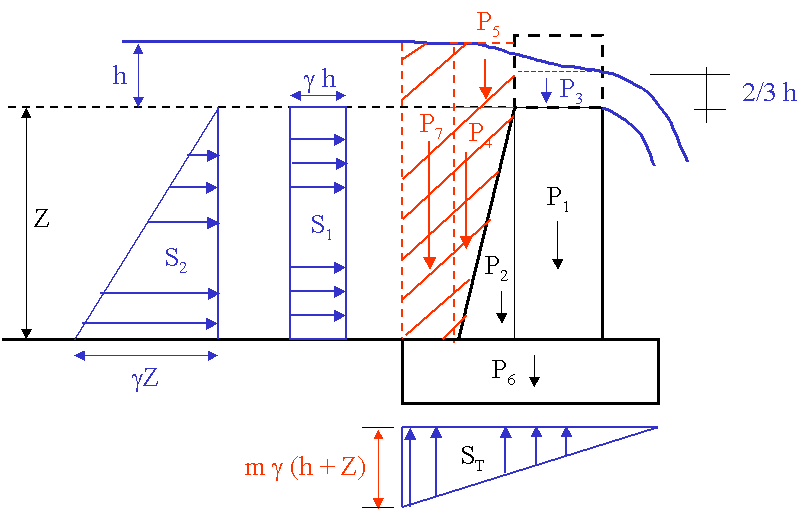
\includegraphics[scale=0.5]{immagini/forze_agenti_briglia.png}
    \caption{Rappresentazione delle forze e dei momenti agenti e reagenti sul profilo della briglia.}
    \label{forze_agenti_briglia}
\end{figure}

\begin{table}[H] \centering
    \caption{\textcolor{red}{Valori relativi alla verifica tradizionale del solo corpo briglia. La sottospinta idraulica viene trascurata, poiché riguarda la fondazione dell'opera.}}
    \begin{tabular}{ccccc}
    \toprule
           & Forze (N) & bracci (m) & Momenti (N m)    &         \\
    \midrule
    P1 (N) & 75744     & 0.60       & 45446.4          &         \\
    P2 (N) & 28404     & 1.50       & 42606            &         \\
    P3 (N) & 9040      & 0.60       & 5424             &         \\
    P4 (N) & 11835     & 1.80       & 21303            &         \\
    P5 (N) & 10170     & 1.65       & 16780.5          &         \\
    somma  & 135193.0  &            & 131559.9         & stab.   \\
    \midrule
    S1 (N) & 29719     & 1.32       & 39080.5        &         \\
    S2 (N) & 34584.5   & 0.88       & 30319.1 &         \\
    somma  & 64303.5   &            & 69399.6          & destab. \\
    \bottomrule
    \end{tabular}
    \end{table}

    \begin{table}[H] \centering
        \caption{\textcolor{red}{Valori relativi alla verifica tradizionale del corpo briglia e della fondazione. In questo caso la sottospinta idraulica viene considerata.}}
        \begin{tabular}{ccccc}
            \toprule
           & Forze (N) & bracci (m) & Momenti (N m)    &         \\
    \midrule
        P1 (N)        & 75744    & 0.60 & 45446.4          &         \\
        P2 (N)        & 28404    & 1.50 & 42606            &         \\
        P3 (N)        & 9040     & 0.60 & 5424             &         \\
        P4 (N)        & 11835    & 1.80 & 21303            &         \\
        P5 (N)        & 10170    & 1.65 & 16780.5          &         \\
        P6 (N)        & 37440    & 1.20 & 44928            &         \\
        P7 (N)        & 11280    & 2.25 & 25380            &         \\
        ST (N) (neg.) & 9024     &      &                  &         \\
        somma         & 174889.0 &      & 201867.9         & stab.   \\
       \midrule
        S1 (N)        & 29719    & 1.97 & 58397.8          &         \\
        S2 (N)        & 34584.5  & 1.53 & 52799.0          &         \\
        ST (N)        &          & 1.60 & 14438            &         \\
        somma         & 64303.5  &      & 125635.2         & destab. \\
        \bottomrule
        \end{tabular}
        \end{table}

Avendo calcolato i valori delle spinte e dei momenti agenti nel sistema, è possibile riportare i risultati della verifica allo scorrimento ed al ribaltamento.
\begin{table}[H] \centering
    \caption{\textcolor{red}{Risultati della verifica a scorrimento e ribaltamento del corpo briglia e del corpo briglia con la fondazione.}}
    \begin{tabular}{cc}
    \toprule
    \multicolumn{2}{c}{CORPO BRIGLIA} \\
    $G_{scorr}$                               & 1.47                 \\
    $G_{rib}$                              & 1.90                 \\
    u (m)                             & 0.460                \\
    e (m)                             & 0.590                \\
    b/3 (m)                           & 0.700                \\
    sigma valle (MPa)                 & 0.173                \\
    sigma monte (MPa)                 & -0.044               \\
    \midrule
    \multicolumn{2}{c}{CORPO+FONDAZIONE}                     \\
    $G_{scorr}$                       & 1.21                 \\
    $G_{rib}$                         & 1.61                 \\
    u (m)                             & 0.436                \\
    e (m)                             & 0.764                \\
    b/3 (m)                           & 0.800                \\
    sezione reagente (m)              & 1.3                  \\
    sigma valle (MPa)                 & 0.267                \\
    sigma monte (MPa)                 & 0.000                \\
    \bottomrule
    \end{tabular}
    \end{table}

La verifica allo scorrimento, secondo il metodo tradizionale, è guidata dalla formula $\Sigma F_{orizz.}<f\cdot\Sigma F_{vert.}$, dove $f$ è il coefficiente di attrito corpo-fondazione o tra la fondazione ed il terreno.\\
Con questa verifica si valuta la tendenza alla traslazione effettuata dalle forze orizzontali agenti sul sistema.\\
Portando la sommatoria delle forze verticali a destra della disequazione, risulta che la verifica è accettata se il rapporto tra le forze (comprendente il coefficiente d'attrito) è superiore a 1. In entrambi i casi, la verifica allo scorrimento risulta soddisfatta.\\
Per quanto riguarda la verifica al ribaltamento, secondo il metodo tradizionale, la formula generale è $G_s = \frac{\Sigma M_{O,stab.}}{\Sigma M_{O,rib.}} \ge 1.5$.\\
Anche per questa verifica, in entrambi i casi la struttura viene considerata sicura.\\
Infine, per quanto riguarda lo schiacciamento, che si manifesta tra corpo briglia e fondazione, e tra la fondazione ed il terreno, la formula generale è $\sigma= \frac{\Sigma F_v}{B} \cdot \left(1 \pm \frac{6 \cdot e}{B}\right)$. Tale tensione calcolata ($\sigma$) dev'essere inferiore rispetto a quella sopportabile dal materiale con cui è fatta l'opera; mentre la tensione ammissibile dal calcestruzzo è 0.35 MPa, quella agente sull'opera è di 0.267 MPa.

\subsubsection{Verifiche NTC-2018 della briglia}
Come anticipato nelle verifiche precedenti, in questa sezione verranno riportati solamente i valori geometrici accettabili secondo la verifica NTC-2018 (Norme Tecniche Costruzione).\\
Tale metodo implica l'utilizzo di coefficienti tabellati, in modo da incrementare l'effetto delle forze destabilizzanti e di ridurre l'effetto stabilizzante sull'opera. Ogni tabella ha un codice proprio, e per ogni caso di studio è frequente trovare una serie di codici, poiché avviene la combinazione dei diversi coefficienti.\\
Si comincia la verifica riportando i valori geometrici (finali e corretti) necessari per svolgere la verifica al ribaltamento della struttura.
\begin{table}[H] \centering
    \caption{\textcolor{red}{Valori dimensionali e coefficienti fisici necessari per effettuare la procedura di verifica al ribaltamento della briglia secondo NTC-2018. Tali valori sono differenti rispetto a quelli di massima stimati inizialmente.}}
    \begin{tabular}{cc}
    \toprule    
        DATI & \\
    \bottomrule
    peso sp. acqua ($N/m^3$)      & 10000 \\
    peso sp. mat. ($N/m^3$)       & 24000 \\
    altezza gaveta: h (m)      & 1.13  \\
    altezza corpo: z(m)        & 2.63  \\
    coronamento: s (m)         & 1.20  \\
    base corpo: b(m)           & 2.30  \\
    base fondazione: $B_f$ (m)    & 2.75  \\
    altezza fondazione: $z_f$ (m) & 0.90  \\
    sporto monte: $s_m$(m)         & 0.45  \\
    sporto valle: $s_v$(m)        & 0.00  \\
    coeff. riduz.sottosp.: m   & 0.20  \\
    \bottomrule
    \label{valori_dimensionali_NTC2018}
    \end{tabular}
\end{table}
La verifica al ribaltamento, secondo i criteri A1, M1 e R3, genera i seguenti risultati.
\begin{table}[H] \centering
    \caption{\textcolor{red}{Valori dei coefficienti, delle forze e dei momenti, necessari per svolgere la verifica al ribaltamento della struttura, secondo le NTC-2018 e criteri A1, M1 e R3.}}
    \begin{tabular}{cccccl}
\toprule
& Coeff. parz. & Forze (N) & bracci (m) & Momenti (N m) &  \\
\midrule
P1 (N) & 0.9                & 68169.6   & 0.60       & 40902 &   \\
P2 (N) & 0.9    & 31244.4   & 1.57       & 48950            &         \\
P3 (N) & 0.9     & 8136      & 0.60       & 4882             &         \\
P4 (N) & 0.9     & 13018.5   & 1.93       & 25169            &         \\
P5 (N) & 0.9         & 11187     & 1.75       & 19577            & \\
P6 (N)       & 0.9   & 53460     & 1.38       & 73508        &         \\
P7 (N) & 0.9       & 15228     & 2.53       & 38451            & \\
ST (N) sottosp. & sfav.		1.5  & 15510     & &  & \\
somma                  &      & 184933.5  &  & 251437.5    & stab.   \\
\midrule
& Coeff. parz. &  &            &    &         \\
S1 (N)      & 1.1                & 32690.9   & 2.22   & 72410.34  & \\
S2 (N) & 1.1     & 38042.9  & 1.78       & 67589.64 &         \\
ST (N) sottosp.        &  &   & 1.83       & 28435            &         \\
somma  &      & 70733.9   &            & 168435.0         & destab. \\
\bottomrule
    \end{tabular}
    \end{table}
Affinché la verifica possa essere considerata accettata, è necessario che il momento reagente (compreso del fattore di correzione) sia superiore rispetto a quello agente.\\
Infatti, per un momento stabilizzante (compreso del coefficiente idoneo) di 218.6 kNm, il momento agente è di 168.4 kNm, per cui la verifica al ribaltamento è soddisfatta.

Successivamente alla verifica al ribaltamento secondo la NTC-2018, è necessario verificare la struttura (corpo e fondazione) alla forza di scorrimento agente.\\
I valori dimensionali con cui è svolta la verifica allo scorrimento sono i medesimi della verifica al ribaltamento secondo la NTC-2018 (riportati nella tabella \ref{valori_dimensionali_NTC2018}).\\
Come per la verifica al ribaltamento, anche quella allo scorrimento viene svolta secondo i coefficienti dei criteri A1, M1 e R3; tali valori generano i seguenti risultati.

\begin{table}[H] \centering
    \caption{\textcolor{red}{Valori dei coefficienti, delle forze e dei momenti, necessari per svolgere la verifica allo scorrimento della struttura (corpo e fondazione), secondo le NTC-2018 e criteri A1, M1 e R3.}}
    \begin{tabular}{cccccl}
\toprule
& Coeff. parz. & Forze (N) & bracci (m) & Momenti (N m) &         \\
\midrule
    P1 (N) & 1.0  & 75744              & 0.60       & 45446 &         \\
    P2 (N) & 1.0  & 34716 & 1.57       & 54388         &         \\
    P3 (N)        & 1.0    & 9040               & 0.60       & 5424 &\\
    P4 (N)        & 1.0 & 14465 & 1.93  & 27966                  & \\
    P5 (N)        & 1.0                & 12430 & 1.75 & 21753    & \\
    P6 (N)        & 1.0   & 59400              & 1.38       & 81675  & \\
    P7 (N)        & 1.0 & 16920 & 2.53       & 42723         & \\
    ST (N) (neg.) & 1.5                & 15510  & -          & -   & \\
    somma         &        & 207205.0   &  & 279375.0  & stab. \\
    \midrule
    & Coeff. parz. & &   &                        &         \\
    S1 (N)        & 1.3 & 38634.7 & 2.22 & 85576                  & \\
    S2 (N)        & 1.3 & 44959.85 & 1.78       & 79879     &         \\
       &       &   & &      &         \\
    somma & & 83594.55  &    & 165454.5               & destab. \\
    \bottomrule
    \end{tabular}
    \end{table}

Affinché la struttura possa essere considerata verificata allo scorrimento, occorre che la componente resistiva della forza sia superiore rispetto a quella agente massima.\\
In questo caso, la componente orizzontale resistente è di 83.9 kN, mentre quella agente è di 83.6 kN; ne consegue che l'opera è dimensionata correttamente a scorrimento.\\

Al fine di analizzare la resistenza totale della struttura secondo le NTC-2018, è necessario valutare il carico limite resistivo.\\
Come per gli altri casi, la sezione di studio è quella tra il corpo della briglia e della fondazione.

\begin{table}[H] \centering
\caption{\textcolor{red}{Valori dei coefficienti, delle forze e dei momenti, necessari per svolgere la verifica al carico limite della struttura (corpo e fondazione), secondo le NTC-2018 e criteri A1, M1 e R3.}}
    \begin{tabular}{cccccl}
\toprule
& Coeff. & Forze (N) & bracci (m) & Momenti (N m) &         \\
\midrule
P1 (N) & 1.0         & 75744     & 0.60       & 45446         &         \\
P2 (N) & 1.0         & 34716     & 1.57       & 54388         &         \\
P3 (N) & 1.0         & 9040      & 0.60       & 5424          &         \\
P4 (N) & 1.0         & 14465     & 1.93       & 27966         &         \\
P5 (N) & 1.0         & 12430     & 1.75       & 21753         &         \\
P6 (N) & 1.0         & 59400     & 1.38       & 81675         &         \\
P7 (N) & 1.0         & 16920     & 2.53       & 42723         &         \\
ST (N) (neg.) & 0.0  & 0.0       & -          & -             &         \\
somma         &      & 222715.0  &            & 279375.0      & stab.   \\
\midrule
& Coeff. &     &            &               &         \\
S1 (N)        & 1.3  & 38634.7   & 2.22       & 85576         &         \\
S2 (N)        & 1.3  & 44959.85  & 1.78       & 79879         &         \\
somma         &      & 83594.6   &            & 165454.5      & destab. \\
\bottomrule
    \end{tabular}
    \end{table}

Come per gli altri casi, affinchè la struttura possa essere considerata resistente alla sollecitazione della verifica, la componente destabilizzante dev'essere inferiore alla componente stabilizzante. In questo caso, la reazione resistente del terreno è pari a 225.8 $kN/m$, mentre la tensione reale verticale che si genera è di 222.7 $kN/m$; ciò implica che la verifica al carico limite è positiva.